%% Beamer Presentation using 16:9 aspect ratio (HDTV standard aspect ratio)
\documentclass[aspectratio=169]{beamer}

%% Metropolis or mtheme Theme
\usetheme{metropolis}

% Packages
\usepackage{fancyvrb}
\usepackage{graphicx}
\usepackage{listings}
\usepackage[]{hyperref, amsmath}
\usepackage{pgfplots}
\usepackage{appendixnumberbeamer}

% Provide an easy command for mono spaced font: \t{text}
\renewcommand{\t}[1]{\texttt{#1}}

% Provide an easy command for full screen graphics
\newcommand<>{\fullsizegraphic}[1]{
{
    \begin{frame}[plain]
        \begin{tikzpicture}[remember picture,overlay]
            \node[at=(current page.center)] {
                \includegraphics[width=\paperwidth]{#1}
            };
        \end{tikzpicture}
    \end{frame}
}
}
\newcommand<>{\fullsizegraphich}[1]{
{
    \begin{frame}[plain]
        \begin{tikzpicture}[remember picture,overlay]
            \node[at=(current page.center)] {
                \includegraphics[height=\paperheight]{#1}
            };
        \end{tikzpicture}
    \end{frame}
}
}

% Customize the Fancy Verbatim environment's default font and margins
\RecustomVerbatimEnvironment
{Verbatim}{Verbatim}
{formatcom=\scriptsize,xleftmargin=0.75ex}

% use filled blocks for default, alert and example blocks
\metroset{block=fill}

% Title format uses smallcaps
\metroset{titleformat=smallcaps}

% 42 Lines logo colors
\definecolor{blue}{RGB}{5,76,111}
\definecolor{lightblue}{RGB}{53,137,175}
\definecolor{grey}{RGB}{187,187,187}

% Adjust Metropolis theme to use 42 Lines colors
\setbeamercolor{alerted text}{fg=lightblue}
\setbeamercolor{example text}{fg=blue}
\setbeamercolor{palette primary}{bg=blue}

% Customization for code listings including font size, a background and margins
\lstset{
    basicstyle=\scriptsize\ttfamily,
    backgroundcolor=\color{normal text.bg!80!normal text.fg!50!normal text.bg},
    frame=single,
    framerule=0pt,
}

% 42 Lines logo in top right corner
\graphicspath{{../../42lines-template/}}
\titlegraphic{\hfill
\includegraphics[width=.15\textwidth]{42-LOGO}}

% Here ends the preamble


\title{Observability Through the Lens of\\Metrics and Events}
%%\subtitle{Subtitle Foo on Bar}
\institute{42 Lines, Inc.}
\author{Jack Neely jjneely@42lines.net\\Breandan Dezendorf breandan@42lines.net}

\date{\today}

\begin{document}

\maketitle

\begin{frame}[fragile]
    \frametitle{What's a Metric?}

    Prometheus:
\begin{lstlisting}
# HELP http_requests_total total HTTP hits
# TYPE http_requests_total counter
http_requests_total 34877
# HELP node_load1 1m load average.
# TYPE node_load1 gauge
node_load1 1.35
\end{lstlisting}

    Graphite:
\begin{lstlisting}
servers.A.http.hits 34877 1234567890
servers.A..collectd.load.load.shortterm 1.35 1234567890
\end{lstlisting}

    OpenTSDB:
\begin{lstlisting}
put http.hits 1234567890 34877 host=A
put proc.loadavg.1min 1234567890 1.35 host=A
\end{lstlisting}
\end{frame}

\begin{frame}
    \frametitle{What's an Event?}

\end{frame}

\begin{frame}
    \frametitle{Graphite's \t{summarize()} and Non-Aligned Data}

    \begin{center}
        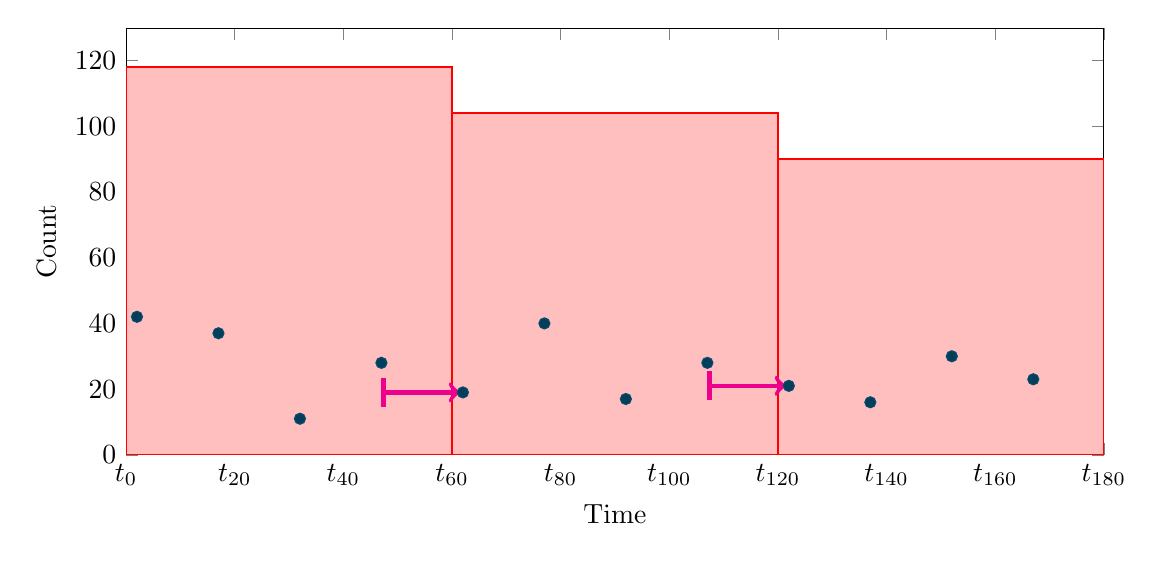
\begin{tikzpicture}[]
            \begin{axis}[
                width=14cm,
                height=7cm,
                xlabel=Time,
                ylabel=Count,
                xticklabel={$t_{\pgfmathprintnumber{\tick}}$},
                xmin=0, ymin=0, xmax=180
            ]
                \addplot+[only marks] coordinates {
                    (2, 42)  % 118
                    (17, 37)
                    (32, 11)
                    (47, 28)
                    (62, 19) % 104
                    (77, 40)
                    (92, 17)
                    (107, 28)
                    (122, 21) % 67+N
                    (137, 16)
                    (152, 30)
                    (167, 23)
                };
                \addplot+[ybar interval,fill=pink,mark=none] coordinates {
                    (0, 118)
                    (60, 104)
                    (120, 90)
                    (180, 0) % ybar interval extra coord
                };
                \draw[ultra thick,magenta,|->,shorten >=1pt] (47,19) to (62,19);
                \draw[ultra thick,magenta,|->,shorten >=1pt] (107,21) to (122,21);
            \end{axis}
        \end{tikzpicture}
    \end{center}
\end{frame}

\begin{frame}[standout]
    Thank You!
\end{frame}

\appendix

\end{document}
